\documentclass[aspectratio=169,11pt]{beamer}
\usepackage[T1]{fontenc}
\usepackage[utf8]{inputenc}
\usepackage{lmodern}
\usepackage{mastering_ir_derivatives_beamer_1.0}
\usepackage{booktabs}
\usepackage{array}
\usepackage{listings}

% Retain the supplied visual system without changing the authored slide count.
\beamerdefaultoverlayspecification{<*>}
\AtBeginSection[]{}
\AtBeginSubsection[]{}

\hypersetup{
    colorlinks=true,
    linkcolor=blue,
    urlcolor=blue
}

\lstset{
    basicstyle=\ttfamily\scriptsize,
    breaklines=true,
    columns=fullflexible
}

\newcommand{\product}{TGIR QuantLib Tools}
\newcommand{\code}[1]{\texttt{#1}}
\newcommand{\docdate}{2026-04-06}


\usepackage[T1]{fontenc}
\usepackage[utf8]{inputenc}
\usepackage{lmodern}
\usepackage{amsmath,amssymb,mathtools}
\usepackage{booktabs,array}
\usepackage{tikz}
\usetikzlibrary{arrows.meta,positioning,calc}
\usepackage{xcolor}

\definecolor{TgirNavy}{HTML}{0B1F2A}
\definecolor{TgirTeal}{HTML}{00A88F}
\definecolor{TgirMint}{HTML}{BFE9DD}
\definecolor{TgirOrange}{HTML}{D06C3B}
\definecolor{TgirPaper}{HTML}{F7F2E8}
\definecolor{TgirGray}{HTML}{61717C}

\setbeameroption{hide notes}
\setbeamersize{text margin left=8mm,text margin right=8mm}

\newcommand{\takeaway}[1]{%
  \vfill
  \begin{beamercolorbox}[rounded=true,sep=1.5mm,wd=\linewidth]{block body}
    \textbf{Takeaway.} #1
  \end{beamercolorbox}}
\newcommand{\src}[1]{\note{[Sources] #1}}
\newcommand{\summaryslide}[6]{%
  \begin{frame}{#1}
    \begin{itemize}\setlength\itemsep{0.9em}
      \item #2
      \item #3
      \item #4
    \end{itemize}
    \takeaway{#5}
    \src{#6}
  \end{frame}}

\begin{document}

% 1
\begin{frame}[plain]
  \begin{tikzpicture}[remember picture,overlay]
    \fill[TgirNavy] (current page.south west) rectangle (current page.north east);
    \fill[TgirTeal] (current page.south west) rectangle ([xshift=10mm]current page.north west);
    \node[anchor=west,text width=.82\paperwidth,align=left] at ([xshift=20mm]current page.west)
    {\usebeamerfont{title}\color{white}Building a QuantLib Derivatives Workbench\par\vspace{4mm}
     \usebeamerfont{subtitle}\color{TgirMint}Human-directed development with Codex and Claude, from swaps to callable XCCY\par\vspace{7mm}
     \color{white!70}\normalsize Tim Launer + two coding agents\hfill Evidence through 22 August 2026};
  \end{tikzpicture}
  \src{Local Git history, GitHub repository metadata, source tree, tests, documentation, and filesystem timestamps.}
\end{frame}

% 2
\begin{frame}{The product and its collaborative method matured together}
  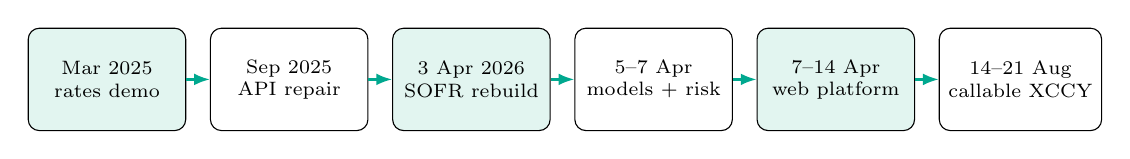
\begin{tikzpicture}[node distance=4mm and 3mm, every node/.style={font=\scriptsize,align=center}]
    \node[draw,rounded corners,fill=TgirMint!45,minimum width=20mm,minimum height=13mm] (a) {Mar 2025\\rates demo};
    \node[draw,rounded corners,fill=white,right=of a,minimum width=20mm,minimum height=13mm] (b) {Sep 2025\\API repair};
    \node[draw,rounded corners,fill=TgirMint!45,right=of b,minimum width=20mm,minimum height=13mm] (c) {3 Apr 2026\\SOFR rebuild};
    \node[draw,rounded corners,fill=white,right=of c,minimum width=20mm,minimum height=13mm] (d) {5--7 Apr\\models + risk};
    \node[draw,rounded corners,fill=TgirMint!45,right=of d,minimum width=20mm,minimum height=13mm] (e) {7--14 Apr\\web platform};
    \node[draw,rounded corners,fill=white,right=of e,minimum width=20mm,minimum height=13mm] (f) {14--21 Aug\\callable XCCY};
    \foreach \x/\y in {a/b,b/c,c/d,d/e,e/f}{\draw[-{Latex[length=2mm]},TgirTeal,thick] (\x) -- (\y);}
  \end{tikzpicture}
  \begin{itemize}\setlength\itemsep{0.8em}
    \item Git records the major releases; local birth times refine the one-commit August implementation sequence.
    \item Tim directed the economics; Codex built most specifications, code, integrations, and tests; Claude added review, validation, and regression depth.
  \end{itemize}
  \takeaway{The repository evolved with the human--agent team: every product increment also strengthened the method used to build the next one.}
  \src{git log --reverse; GitHub pull requests 1--3; local stat birth times.}
\end{frame}

% 3
\summaryslide{A pricer is a disciplined cash-flow machine}
{The product defines dated, signed cash flows and exercise rights; the market supplies curves, volatility, FX, correlations, and fixings.}
{The model maps uncertainty into state dynamics; the numerical method converts those dynamics into values and risks.}
{Dates, currencies, day counts, collateral, quote conventions, and measures are economic inputs rather than metadata.}
{Sophisticated numerics cannot repair an incorrectly specified contract.}
{QuantLib documentation; repository architecture and pricing specifications.}

% 4
\summaryslide{The first demo became a corrected QuantLib composition}
{The March 2025 release connected a simple curve, swap, European swaption, and Bermudan through Python bindings.}
{The initial Bermudan incorrectly used a European Black engine and an unsuitable underlying swap definition.}
{September repairs introduced a forward-starting underlying and Hull--White \texttt{TreeSwaptionEngine}, while fixing changed QuantLib APIs.}
{Compact examples become reliable only when product, engine, conventions, and smoke tests agree.}
{Commits 8e17f9f, 6bea9e2, and 21a994f; GitHub pull requests 1 and 2.}

% 6
\begin{frame}{SOFR curve construction became a tested calibration}
  \begin{columns}[T,onlytextwidth]
    \column{.49\textwidth}
    \textbf{Market construction}\par\medskip
    Overnight front point plus SOFR OIS helpers spanning short tenors to 30 years; log-cubic discount interpolation and explicit settlement conventions.
    \column{.47\textwidth}
    \textbf{Evidence}\par\medskip
    Every helper reprices to its quote; discount, zero, and one-day forward views expose curve shape and interpolation behavior.
  \end{columns}
  \takeaway{The curve is a calibrated market object with residuals, not merely a line drawn through rates.}
  \src{Commit abfe66f; portfolio.py build\_sofr\_curve; tests/test\_sofr\_curve.py.}
\end{frame}

% 7
\summaryslide{European swaptions calibrate the short-rate model}
{A diagonal strip maps each future exercise date to the tenor of its remaining swap.}
{Normal-volatility quotes become QuantLib swaption helpers priced with a Jamshidian engine under Hull--White.}
{Mean reversion is governed; a constant volatility minimizes declared helper pricing errors and reports every residual.}
{Calibration is reproducible only when helper selection, units, objective, bounds, and stopping rules are visible.}
{Commit 31df798; portfolio.py calibration routines; model documentation and tests.}

% 8
\begin{frame}{Bermudan pricing uses backward induction}
  \[
    V(t_i,x)=\max\!\left(E(t_i,x),\;
    \mathbb E\!\left[D_{i,i+1}V(t_{i+1},X_{i+1})\mid X_i=x\right]\right).
  \]
  \begin{itemize}\setlength\itemsep{0.8em}
    \item Hull--White contributes a one-dimensional Gaussian short-rate state and an exact fit to today's curve.
    \item A recombining lattice propagates continuation values backward across business-day-adjusted exercise dates.
    \item Tree steps are a numerical parameter and require convergence checks.
  \end{itemize}
  \takeaway{The tree is natural for a single-currency, one-factor stopping problem, not a universal callable engine.}
  \src{QuantLib TreeSwaptionEngine; Hull--White model; repository Bermudan pricing and tests.}
\end{frame}

% 8
\summaryslide{Model comparison, Greeks, and cliquets broadened challenge}
{G2++ added a second Gaussian rates model; governed curve, volatility, and parameter bumps exposed calibration dependency.}
{An SPX cliquet added Black--Scholes forward-start values, analytic Greeks, Monte Carlo distributions, and path-dependent scheduling.}
{Parity, decomposition, scenario, common-random-number, and bump tests checked signs, scaling, and nonlinear response.}
{New products mattered because they expanded the repository's validation vocabulary, not merely its menu.}
{Commits 31df798, aa50775, and 7e08907; portfolio.py and tests.}

% 9
\begin{frame}{A small technical stack became the agents' shared workbench}
  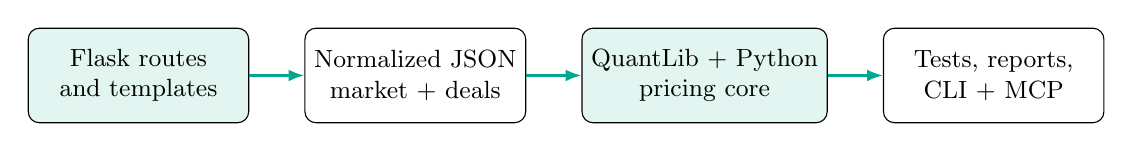
\begin{tikzpicture}[node distance=7mm, every node/.style={font=\small,align=center}]
    \node[draw,rounded corners,fill=TgirMint!45,minimum width=28mm,minimum height=12mm] (ui) {Flask routes\\and templates};
    \node[draw,rounded corners,fill=white,right=of ui,minimum width=28mm,minimum height=12mm] (state) {Normalized JSON\\market + deals};
    \node[draw,rounded corners,fill=TgirMint!45,right=of state,minimum width=28mm,minimum height=12mm] (price) {QuantLib + Python\\pricing core};
    \node[draw,rounded corners,fill=white,right=of price,minimum width=28mm,minimum height=12mm] (diag) {Tests, reports,\\CLI + MCP};
    \foreach \x/\y in {ui/state,state/price,price/diag}{\draw[-{Latex[length=2mm]},TgirTeal,thick] (\x) -- (\y);}
  \end{tikzpicture}
  \begin{itemize}\setlength\itemsep{0.8em}
    \item On the Mac, Git makes Codex and Claude changes, specifications, diffs, tests, JSON evidence, and server logs mutually inspectable.
    \item QuantLib supplies proven C++ primitives; Python makes the extension transparent; Apache, Gunicorn, and systemd run it on DigitalOcean.
  \end{itemize}
  \takeaway{One repository connects human direction, two agents, open-source quant infrastructure, local evidence, and hosted execution.}
  \src{docs/ARCHITECTURE.md; app factory, routes, deployment files, and GitHub Actions history.}
\end{frame}

% 10
\begin{frame}{Tim and two coding agents share one governed Mac workspace}
  \centering
  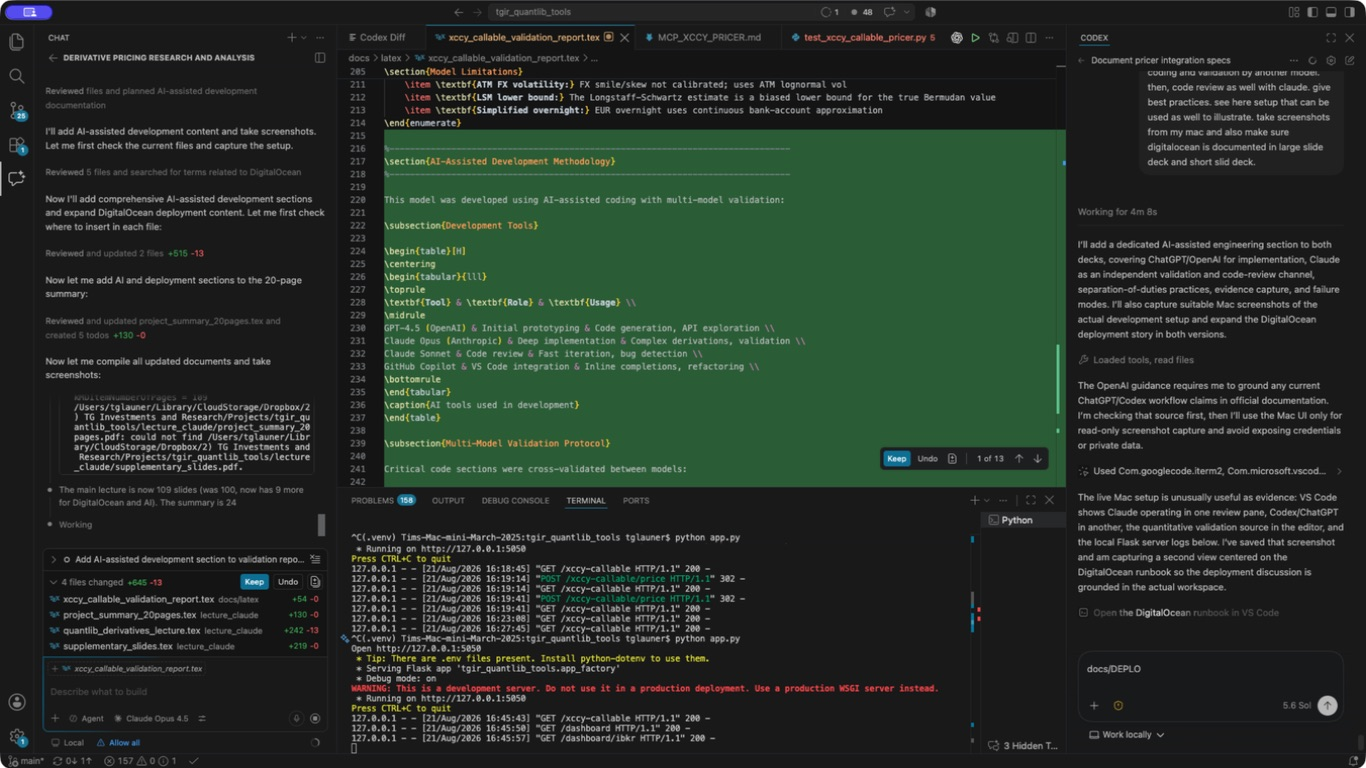
\includegraphics[height=47mm]{assets/mac_cross_model_review_setup.jpg}
  \takeaway{This is where Tim guides, Codex builds, Claude reviews and extends validation, and all three inspect the same source and evidence.}
  \src{Mac screenshot captured 2026-08-21 from the user's VS Code workspace; no secrets shown.}
\end{frame}

% 11
\begin{frame}{One prompt can run the complete delivery chain}
  \centering
  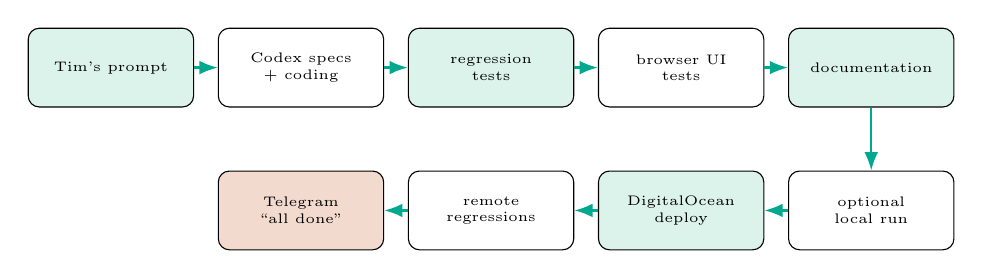
\begin{tikzpicture}[node distance=3mm and 3mm,every node/.style={font=\tiny,align=center}]
    \node[draw,rounded corners,fill=TgirMint!55,minimum width=21mm,minimum height=10mm] (prompt) {Tim's prompt};
    \node[draw,rounded corners,fill=white,right=of prompt,minimum width=21mm,minimum height=10mm] (code) {Codex specs\\+ coding};
    \node[draw,rounded corners,fill=TgirMint!55,right=of code,minimum width=21mm,minimum height=10mm] (test) {regression\\tests};
    \node[draw,rounded corners,fill=white,right=of test,minimum width=21mm,minimum height=10mm] (browser) {browser UI\\tests};
    \node[draw,rounded corners,fill=TgirMint!55,right=of browser,minimum width=21mm,minimum height=10mm] (docs) {documentation};
    \node[draw,rounded corners,fill=white,below=8mm of docs,minimum width=21mm,minimum height=10mm] (local) {optional\\local run};
    \node[draw,rounded corners,fill=TgirMint!55,left=of local,minimum width=21mm,minimum height=10mm] (deploy) {DigitalOcean\\deploy};
    \node[draw,rounded corners,fill=white,left=of deploy,minimum width=21mm,minimum height=10mm] (remote) {remote\\regressions};
    \node[draw,rounded corners,fill=TgirOrange!25,left=of remote,minimum width=21mm,minimum height=10mm] (telegram) {Telegram\\``all done''};
    \foreach \x/\y in {prompt/code,code/test,test/browser,browser/docs,docs/local,local/deploy,deploy/remote,remote/telegram}{\draw[-{Latex},thick,TgirTeal] (\x)--(\y);}
  \end{tikzpicture}
  \vspace{3mm}
  \takeaway{No manual handoff is required after the prompt; Claude's validation extensions and remote regressions protect later Codex changes.}
  \src{User-described operating workflow; repository tests, browser UI, documentation, and DigitalOcean assets. Telegram orchestration is external to this repository.}
\end{frame}

% 12
\begin{frame}{DigitalOcean keeps production deliberately small}
  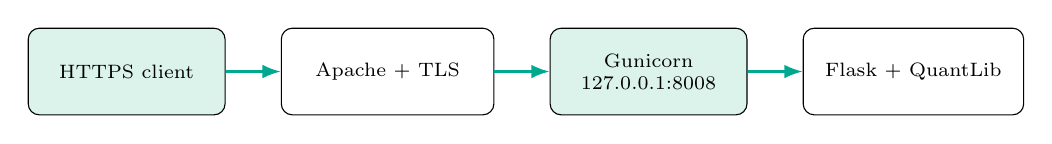
\begin{tikzpicture}[node distance=7mm,every node/.style={font=\scriptsize,align=center}]
    \node[draw,rounded corners,fill=TgirMint!55,minimum width=25mm,minimum height=11mm] (web) {HTTPS client};
    \node[draw,rounded corners,fill=white,right=of web,minimum width=27mm,minimum height=11mm] (apache) {Apache + TLS};
    \node[draw,rounded corners,fill=TgirMint!55,right=of apache,minimum width=25mm,minimum height=11mm] (gunicorn) {Gunicorn\\127.0.0.1:8008};
    \node[draw,rounded corners,fill=white,right=of gunicorn,minimum width=28mm,minimum height=11mm] (app) {Flask + QuantLib};
    \foreach \x/\y in {web/apache,apache/gunicorn,gunicorn/app}{\draw[-{Latex},thick,TgirTeal] (\x)--(\y);}
  \end{tikzpicture}
  \begin{itemize}\setlength\itemsep{0.65em}
    \item systemd runs the app under \texttt{www-data} at \texttt{/var/www/html/tgir\_quantlib\_tools}; secrets stay in a mode-600 \texttt{.env}.
    \item Deployment builds a fresh final-path virtualenv, restarts the service, checks loopback and public TLS health, and rolls back on failure.
  \end{itemize}
  \takeaway{For about USD 7/month, this serious hobby gains a hosted evidence lane with TLS, process, health-check, regression, and rollback controls.}
  \src{docs/DEPLOYMENT.md; GitHub deploy workflow; Apache and systemd templates.}
\end{frame}

% 13
\begin{frame}{QuantLib lacks a native callable XCCY engine}
  \begin{columns}[T,onlytextwidth]
    \column{.48\textwidth}
    \textbf{Native building blocks}\par\medskip
    Curves, calendars, schedules, XCCY swaps, Hull--White/G2, swaption helpers and engines, stochastic processes, and Gaussian path generators.
    \column{.48\textwidth}
    \textbf{Missing composition}\par\medskip
    A domestic-measure joint rates/FX process, callable cross-currency cash-flow semantics, and a multi-date optimal-stopping engine.
  \end{columns}
  \takeaway{Native support is a spectrum: reuse mature primitives while owning the missing economics.}
  \src{QuantLib 1.43 source and documentation; repository callable XCCY assessment.}
\end{frame}

% 14
\summaryslide{The benchmark deal fixes the economic question}
{The example is a ten-year EUR/USD constant-notional swap, non-callable for two years and then annually cancellable.}
{The holder receives quarterly compounded EUR ESTR and pays semiannual USD fixed at 4\%.}
{USD 100 million and EUR 90.909 million notionals exchange initially and finally; USD is collateral and reporting currency.}
{Exercise means cancelling the remaining tail under explicit event ordering, not receiving a generic option payoff.}
{data/xccy\_deal\_10y\_nc2.json; deal schema; callable XCCY pricing specification.}

% 15
\begin{frame}{The hybrid model couples two rates factors with FX}
  \[
  \begin{aligned}
    dr_d &= [\theta_d(t)-a_dr_d]dt+\sigma_d\,dW_d,\\
    dr_f &= [\theta_f(t)-a_fr_f-\rho_{fS}\sigma_f\sigma_S(t)]dt+\sigma_f\,dW_f,\\
    d\log S &= [r_d-r_f-\tfrac12\sigma_S^2(t)]dt+\sigma_S(t)\,dW_S.
  \end{aligned}
  \]
  \begin{itemize}\setlength\itemsep{0.7em}
    \item Dynamics are under the USD money-market measure with $S=$ USD per EUR.
    \item The full $3\times3$ Brownian correlation matrix must be positive semidefinite.
  \end{itemize}
  \takeaway{FX quotation and numeraire determine both the FX drift and the sign of the foreign quanto correction.}
  \src{Callable XCCY quantitative model summary; standalone_xccy_pricer.py; Brigo and Mercurio.}
\end{frame}

% 16
\summaryslide{Calibration separates curves, rates vol, and FX vol}
{USD SOFR discounts domestic cash flows; EUR ESTR forecasts coupons; FX forwards imply the USD-collateralized effective EUR discount curve.}
{One constant Hull--White sigma per currency fits diagonal normal swaptions with governed mean reversions.}
{Piecewise FX sigmas reproduce selected ATM Black maturities after including stochastic-rate contributions to terminal log-FX variance.}
{The exact relative RMS price error and instrument-level residuals disclose the cost of the fixed-volatility approximation.}
{Market JSON, QuantLib calibration helpers, pricing result, and model validation report.}

% 17
\summaryslide{Exact Gaussian transitions control Monte Carlo bias}
{The state contains both Hull--White factors, log FX, and the integrated domestic short rate.}
{Each interval uses exact Ornstein--Uhlenbeck decay and an integrated covariance matrix; eigenfactorization handles near-singular cases.}
{The event grid contains coupon, fixing, payment, notional, exercise, and volatility-bucket dates, with intermediate step caps.}
{Exact conditional transitions reduce discretization bias but do not eliminate sampling error or model risk.}
{standalone_xccy_pricer.py simulation engine; numerical tests and convergence diagnostics.}

% 18
\begin{frame}{Two-pass LSM separates policy learning from pricing}
  \begin{enumerate}\setlength\itemsep{0.75em}
    \item Simulate training paths and move backward through the annual call dates.
    \item Regress discounted future cancellable-tail value on standardized rates, log FX, leg values, squares, and cross-products.
    \item For zero-fee cancellation, exercise when estimated continuation value is negative.
    \item Freeze the policy and apply it forward on an independently seeded pricing sample.
  \end{enumerate}
  \takeaway{Out-of-sample policy valuation removes in-sample look-ahead optimism and reports an honest lower-bound estimate.}
  \src{Longstaff and Schwartz (2001); standalone XCCY implementation and tests.}
\end{frame}

% 19
\begin{frame}{The pricer and its validation framework can evolve together}
  \begin{columns}[T,onlytextwidth]
    \column{.48\textwidth}
    \textbf{Research evidence}\par\medskip
    Stored callable NPV is near USD 8.34 million versus non-callable NPV near USD 0.69 million. Residuals, martingales, exercise profiles, convergence, and bump stability qualify the mark.
    \column{.48\textwidth}
    \textbf{Collaborative engineering path}\par\medskip
    Codex extends the specified core; Claude's regression layer challenges changes; Python keeps evidence transparent, while profiled C++ can add native QuantLib types and scalable simulation.
  \end{columns}
  \takeaway{The system is designed to extend QuantLib rigorously: stabilize economics and tests first, then migrate measured bottlenecks to C++.}
  \src{result.json; validation report; repository architecture; REST integration specification.}
\end{frame}

% 20
\begin{frame}[plain]
  \begin{tikzpicture}[remember picture,overlay]
    \fill[TgirNavy] (current page.south west) rectangle (current page.north east);
    \node[anchor=west,text width=.78\paperwidth,align=left] at ([xshift=22mm]current page.west)
    {\color{TgirMint}\large The compounding achievement\par\vspace{4mm}
     \color{white}\fontsize{23}{28}\selectfont\bfseries
     Tim directs $\rightarrow$ Codex specifies and builds\par
     $\rightarrow$ Claude reviews and extends validation\par
     $\rightarrow$ Mac proves $\rightarrow$ DigitalOcean hosts\par\vspace{5mm}
     \color{white!75}\normalsize A serious hobby: rigorous quantitative engineering from one prompt to tested deployment and a Telegram ``all done''---for about USD 7/month.};
  \end{tikzpicture}
  \src{Synthesis of repository chronology and current validation status.}
\end{frame}

\end{document}
